\documentclass{beamer}

\usepackage{amsmath, amssymb}
% --- CODE LISTING SETUP FOR PYTHON ---
% --- REQUIRED PACKAGES FOR CUSTOM SLIDES ---

% 1. For the Animation Pipeline Flowchart (TikZ)
\usepackage{tikz}
\usetikzlibrary{positioning, arrows.meta, shapes.geometric}

% 2. For the Python Code Styling (Listings)
\usepackage{listings}
\usepackage{xcolor}

% Define custom colors for professional Python highlighting
\definecolor{codegreen}{rgb}{0,0.6,0}
\definecolor{codegray}{rgb}{0.5,0.5,0.5}
\definecolor{codepurple}{rgb}{0.58,0,0.82}
\definecolor{backcolour}{rgb}{0.95,0.95,0.92}

% Set the Python style
\lstdefinestyle{pythonstyle}{
    backgroundcolor=\color{backcolour},   
    commentstyle=\color{codegreen}\itshape,
    keywordstyle=\color{blue}\bfseries,
    numberstyle=\tiny\color{codegray},
    stringstyle=\color{codepurple},
    basicstyle=\ttfamily\scriptsize, % Monospace font to align characters
    breakatwhitespace=false,         
    breaklines=true,                 
    captionpos=b,                    
    keepspaces=true,                 % STRICTLY keeps Python indentation
    numbers=none,                    
    showspaces=false,                
    showstringspaces=false,
    showtabs=false,                  
    tabsize=4
}
\lstset{style=pythonstyle}

\usetheme{Madrid}

\title{A Python based approach to \\ animate geometry and data}
\author[Shubham Tiwari]{
    Shubham Tiwari \\
    22021563022\\
    \vspace{0.3cm}
    \footnotesize Supervisor: Dr. J. V. Ramani \\
    \footnotesize Co-Supervisor: Ms. Ishver Rani Manchanda
}
\institute{Dyal Singh College, University of Delhi}
\date{April 2026}

\begin{document}

%------------------------------------------------
\frame{\titlepage}

%------------------------------------------------
\begin{frame}{Project Abstract}
\begin{itemize}
    \item \textbf{Framework:} Python-based computational environment for converting static equations into interactive animations.
    \item \textbf{Stack:} Leverages \texttt{NumPy} for vectorized array processing and \texttt{Matplotlib} as the rendering engine.
    \item \textbf{Scope:} Covers 2D kinematics, $L_p$ norm morphing, and complex 3D differential topology (Minimal surfaces like Boy's Surface).
    \item \textbf{Goal:} Enhancing student understanding of abstract spatial transformations through visualization.
\end{itemize}
\end{frame}



%------------------------------------------------
%------------------------------------------------
\begin{frame}{Project Motivation: The Visualization Problem}
\begin{itemize}
    \item \textbf{The Gap:} Transitioning from basic mathematics to more abstract concepts (Trigonometry/Calculus/Algebra) often leads to a loss of interest due to lack of intuition.
    \item \textbf{The Solution:} Animation fills the gap between theory and understanding by showing \textit{how} shapes evolve.
\end{itemize}
\vspace{0.3cm}
\begin{quote}
    "The most important thing a mathematician can do is to show that mathematics is a human activity... one of the most creative fields." --- William Thurston
\end{quote}
\end{frame}

%------------------------------------------------
%------------------------------------------------
\begin{frame}{Proof of Publication}
\begin{columns}
\column{0.5\textwidth}
    \textbf{Acceptance Letter}
    \begin{itemize}
        \item \textbf{Title:} "Introduction: Escaping the Static Chalkboard"
        \item \textbf{Publisher:} AkiNik Publications
        \item \textbf{Book:} Research Trends in Mathematics and Statistics (Vol. 35)
        \item \textbf{Date:} April 25, 2026
    \end{itemize}
\column{0.5\textwidth}
    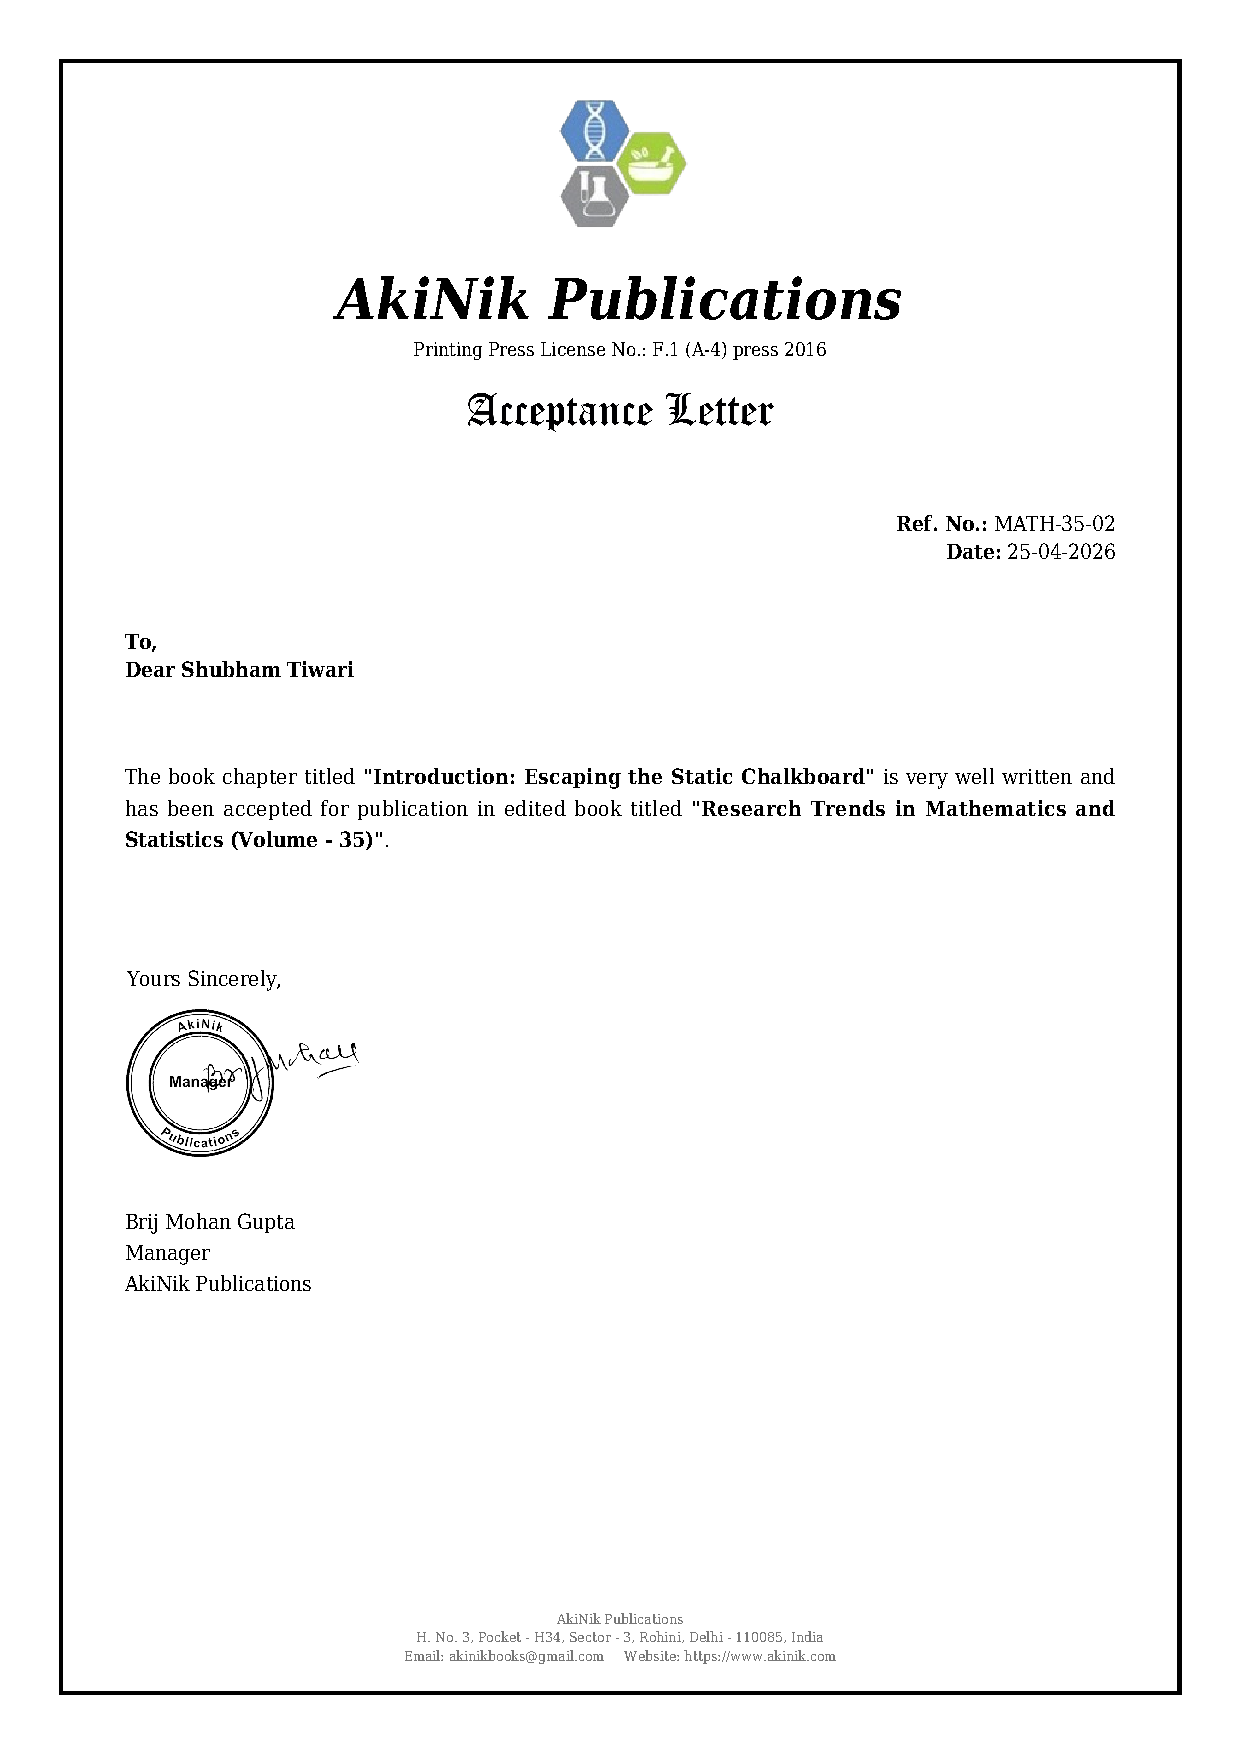
\includegraphics[width=\linewidth, height=0.7\textheight, keepaspectratio]{Acceptance_letter.pdf}
\end{columns}
\end{frame}

%------------------------------------------------
\begin{frame}{Conference Participation}
\begin{columns}
\column{0.5\textwidth}
    \textbf{SCA-2026 Presentation}
    \begin{itemize}
        \item \textbf{Conference:} Int. Conf. on Scientific Computing and its Applications.
        \item \textbf{Host:} South Asian University, New Delhi.
        \item \textbf{Paper:} "A Python-Based Approach for Animating Geometric Concepts..."
    \end{itemize}
\column{0.5\textwidth}
    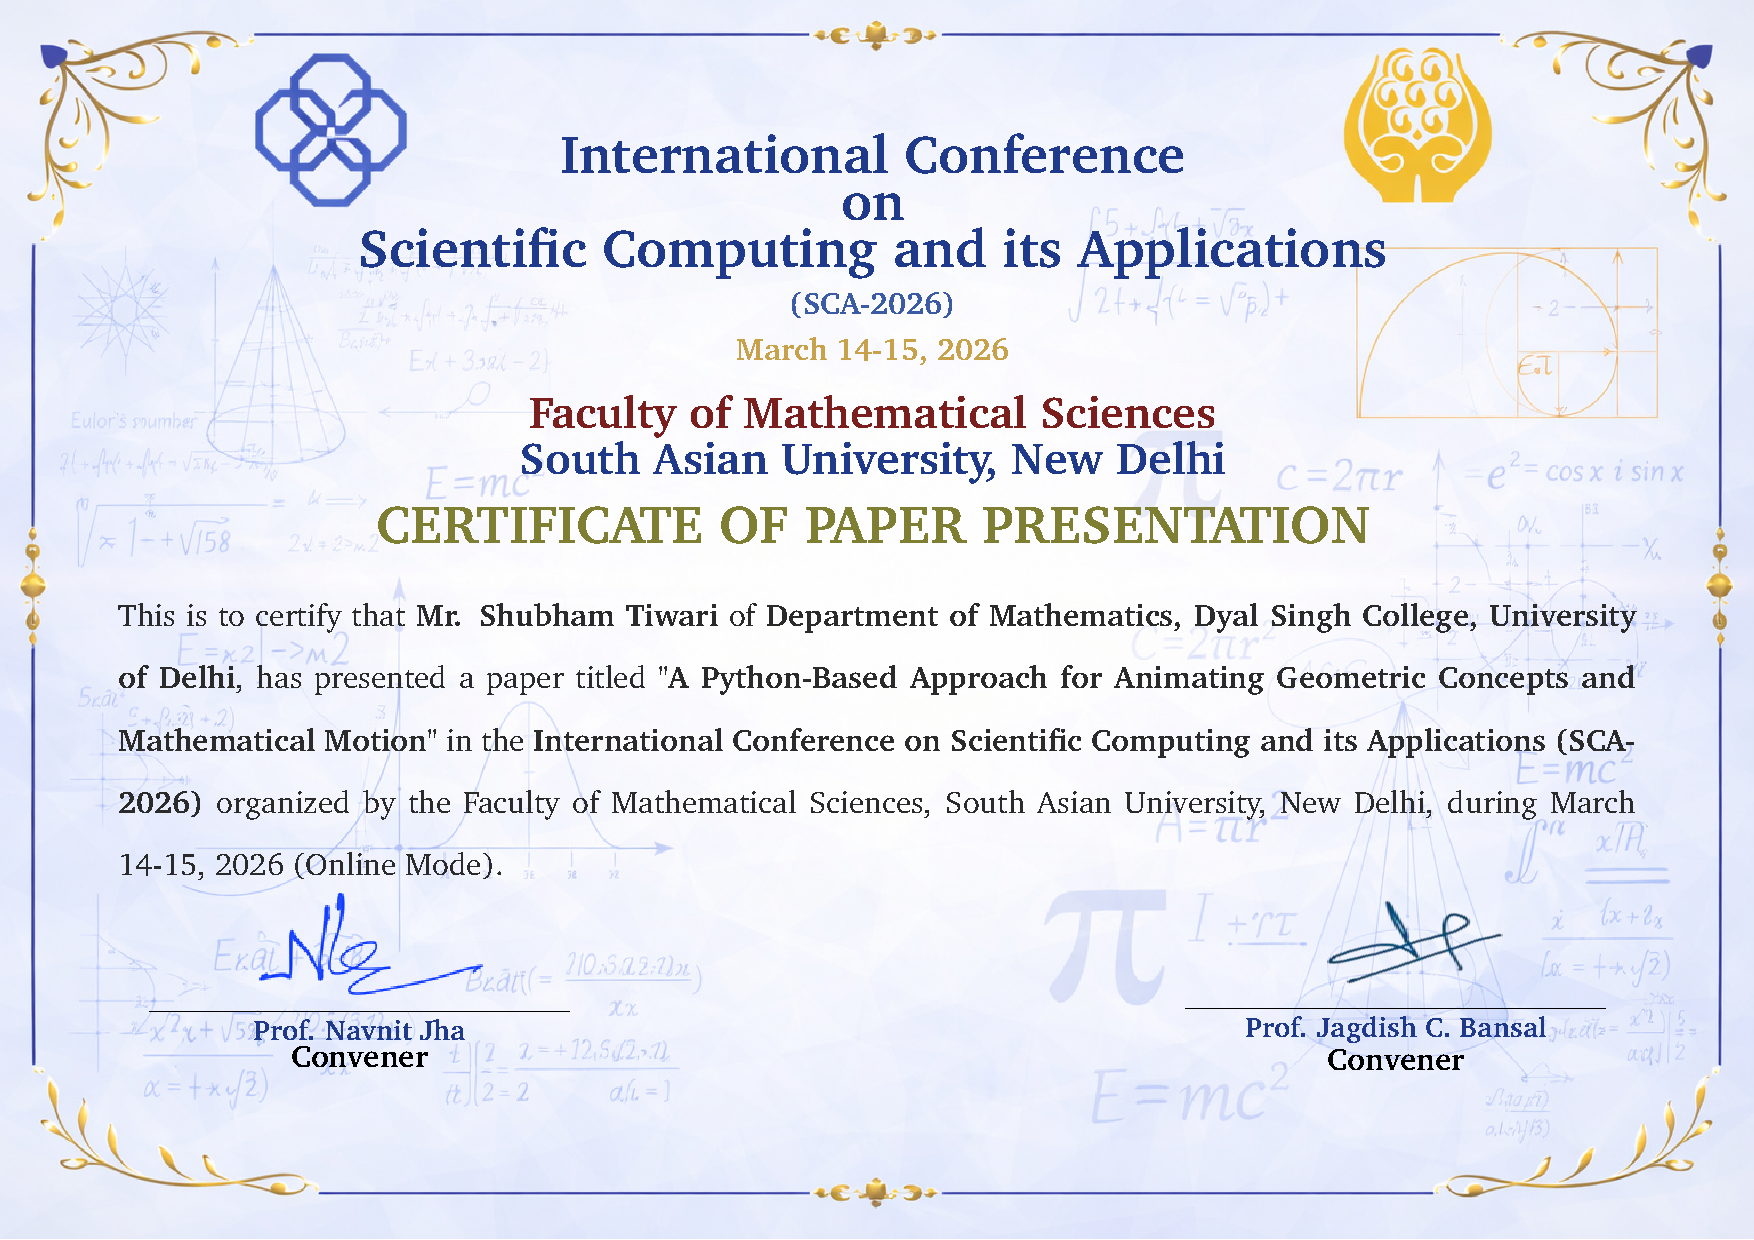
\includegraphics[width=\linewidth, height=0.7\textheight, keepaspectratio]{Participation_certificate.pdf}
\end{columns}
\end{frame}

%------------------------------------------------
\begin{frame}{Research Progress: Monthly Reviews}
\begin{columns}
\column{0.5\textwidth}
    \begin{itemize}
        \item \textbf{Jan:} Initial 3D logic.
        \item \textbf{Feb:} 3D Surface Rendering.
        \item \textbf{Mar:} Topological Morphing.
        \item \textbf{Apr:} Final Review & Conclusion.
    \end{itemize}
\column{0.5\textwidth}
    \begin{figure}
        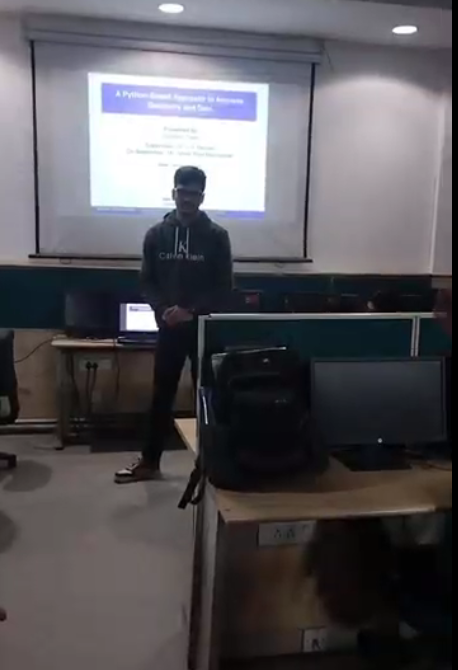
\includegraphics[width=0.45\linewidth]{JAN.png} \hfill
        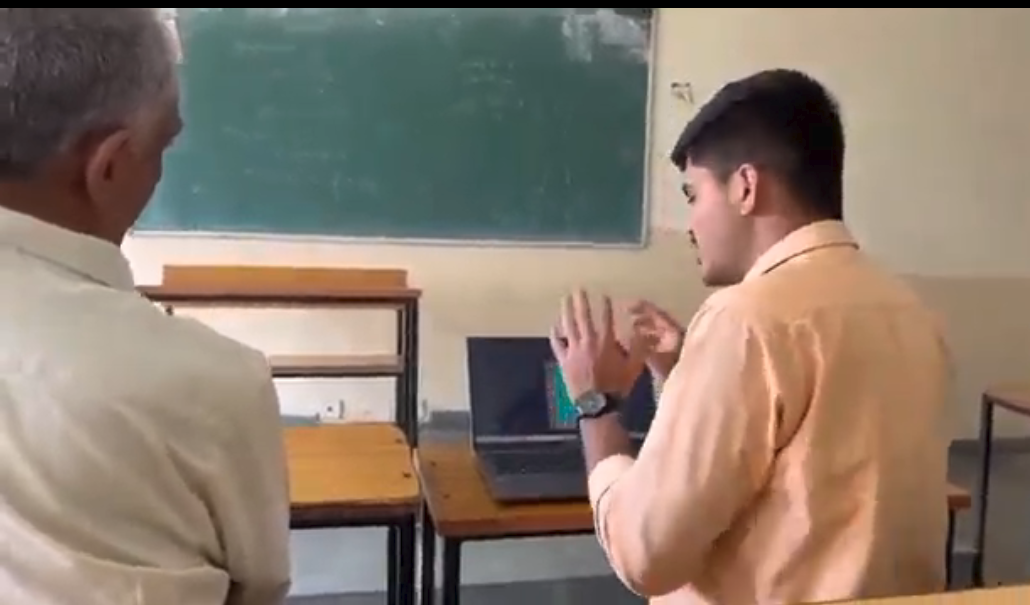
\includegraphics[width=0.45\linewidth]{MAR.png} \\ \vspace{0.2cm}
        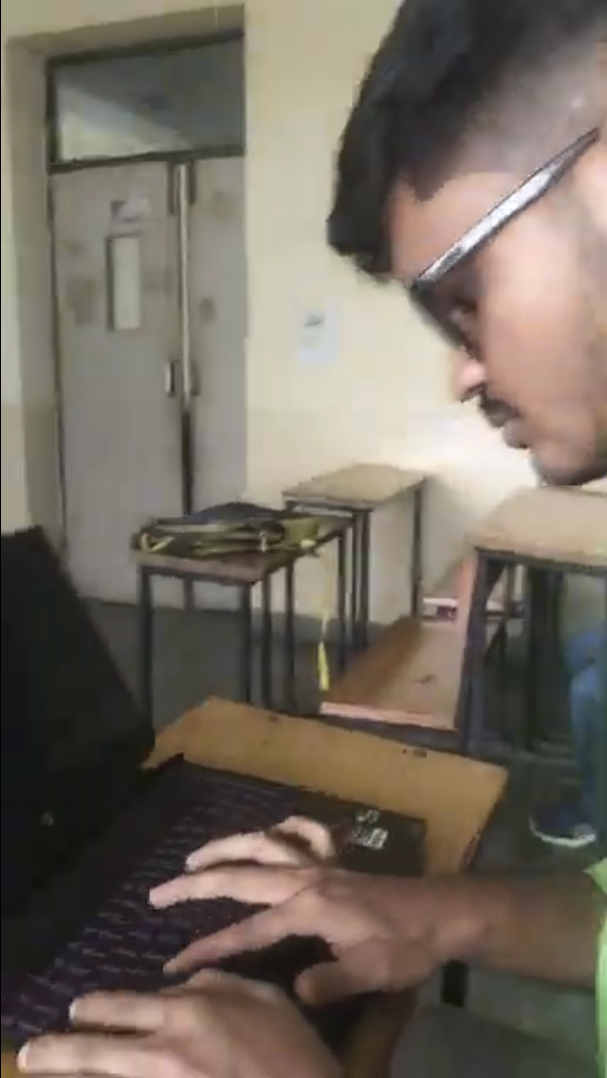
\includegraphics[width=0.45\linewidth]{FEB.png} \hfill
        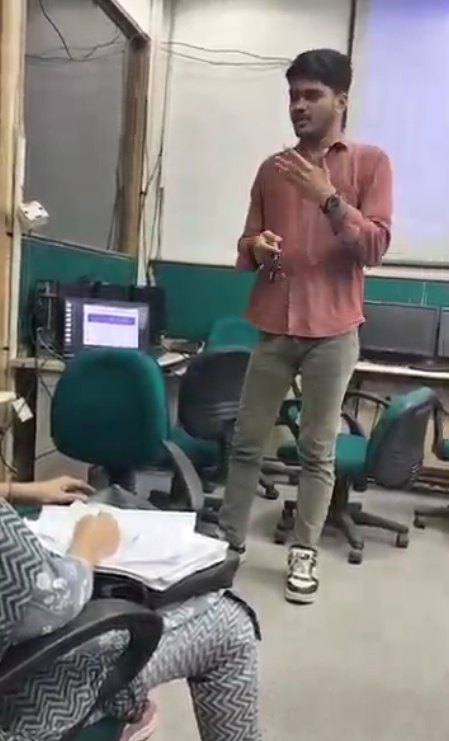
\includegraphics[width=0.45\linewidth]{APR.png}
    \end{figure}
\end{columns}
\end{frame}

%------------------------------------------------
\begin{frame}{Core Idea}
\[
P(t) = (x(t), y(t), z(t))
\]

\begin{itemize}
\item Time introduces motion
\item Geometry defines structure
\item Transformation controls behavior
\end{itemize}

\vspace{0.5cm}
\centering
\textbf{Animation = Geometry + Transformation + Time} \cite{python}
\end{frame}

%------------------------------------------------
\begin{frame}{Parametrization}
\[
x = f(t), \quad y = g(t)
\]

\begin{itemize}
\item Converts static equations into motion \cite{loney}
\item Fundamental tool for curves
\end{itemize}

\vspace{0.3cm}
\textbf{[Show curve tracing animation here]} \cite{matplotlib}
\end{frame}

%------------------------------------------------
\begin{frame}{Sliding Ladder Problem}
\[
x^2 + y^2 = L^2
\]

\[
x = L\cos\theta, \quad y = L\sin\theta
\]

Midpoint:
\[
\left(\frac{L}{2}\cos\theta, \frac{L}{2}\sin\theta \right)
\]

\[
x^2 + y^2 = \left(\frac{L}{2}\right)^2 \quad \cite{loney}
\]

\centering
\textbf{Midpoint traces a circle}

\vspace{0.3cm}
\textbf{[Show ladder animation here]}
\end{frame}

%------------------------------------------------
\begin{frame}{From 2D to 3D}
\[
P' = RP + T
\]

\begin{itemize}
\item $R$ : rotation matrix
\item $T$ : translation vector
\end{itemize}

\vspace{0.3cm}
\textbf{[Show rotating cube animation here]} \cite{friedberg}
\end{frame}

%------------------------------------------------
\begin{frame}{Rotation Matrix}
\[
R_z(\theta) =
\begin{bmatrix}
\cos\theta & -\sin\theta & 0 \\
\sin\theta & \cos\theta & 0 \\
0 & 0 & 1
\end{bmatrix}
\]

\begin{itemize}
\item Preserves distance
\item Preserves angles
\item Defines rigid motion \cite{friedberg}
\end{itemize}

\centering
\textbf{Linear algebra controls space}
\end{frame}

%------------------------------------------------
\begin{frame}{Distance Preservation of Rotation Matrices}
Let $P' = RP$ be the rotated vector. The squared norm of the rotated vector is:
\[
\|P'\|^2 = (RP)^T(RP)
\]

Expanding the transpose:
\[
\|P'\|^2 = P^TR^TRP
\]

Since the rotation matrix is orthogonal, $R^TR = I$, we obtain:
\[
\|P'\|^2 = P^TIP = P^TP
\]

Thus:
\[
\|P'\| = \|P\| \quad \cite{friedberg}
\]

\begin{itemize}
\item Rotation preserves magnitude
\item Distance from origin remains constant
\item Shape does not deform
\end{itemize}
\end{frame}

%------------------------------------------------
\begin{frame}{The Power of Orthogonality in Animation}

The orthogonal property $R^TR = I$ (meaning $R^{-1} = R^T$) is computationally profound:

\vspace{0.3cm}
\begin{itemize}
\item \textbf{Computational Efficiency:} Finding an inverse matrix is usually expensive. For orthogonal rotation matrices, reversing a rotation is just a simple matrix transpose, making frame-by-frame rendering incredibly fast \cite{numpy}.
\vspace{0.2cm}
\item \textbf{Rigid Body Integrity:} Because length and angles are preserved, 3D models do not stretch, shear, or distort during complex tumbling \cite{friedberg}.
\vspace{0.2cm}
\item \textbf{Numerical Stability:} Repeated matrix multiplications can accumulate floating-point errors. Orthogonal matrices naturally resist degradation over time in continuous simulations.
\end{itemize}

\end{frame}
%------------------------------------------------
% --- SLIDE 1: STEPS 1 & 2 ---
\begin{frame}{The Animation Pipeline I: Theory to Data}
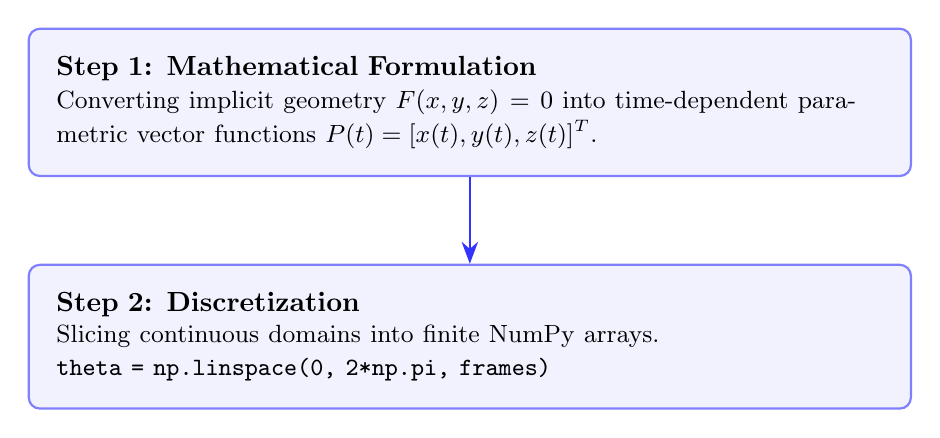
\begin{tikzpicture}[
    node distance=1.1cm,
    box/.style={rectangle, draw=blue!50, thick, fill=blue!5, text width=10.5cm, align=left, rounded corners, minimum height=1.5cm, inner sep=10pt},
    arrow/.style={-{Stealth[scale=1.2]}, thick, draw=blue!80}
]

% Step 1
\node (step1) [box] {
    \textbf{Step 1: Mathematical Formulation} \\
    \small Converting implicit geometry $F(x,y,z)=0$ into time-dependent parametric vector functions $P(t) = [x(t), y(t), z(t)]^T$.
};

% Step 2
\node (step2) [box, below=of step1] {
    \textbf{Step 2: Discretization} \\
    \small Slicing continuous domains into finite NumPy arrays. \\
    \texttt{theta = np.linspace(0, 2*np.pi, frames)}
};

% Connecting Arrow
\draw [arrow] (step1) -- (step2);

\end{tikzpicture}

\vspace{0.4cm}
\begin{itemize}
    \item \textbf{Vectorization:} Applying functions to entire arrays at once for performance.
    \item \textbf{Discrete Mapping:} Finding the optimal $\Delta t$ to balance smoothness vs. speed.
\end{itemize}
\end{frame}

% --- SLIDE 2: STEPS 3 & 4 ---
\begin{frame}{The Animation Pipeline II: Data to Motion}
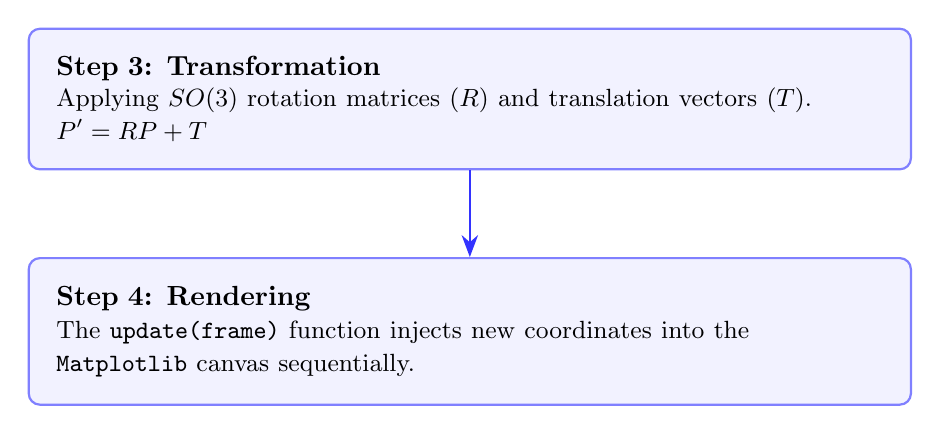
\begin{tikzpicture}[
    node distance=1.1cm,
    box/.style={rectangle, draw=blue!50, thick, fill=blue!5, text width=10.5cm, align=left, rounded corners, minimum height=1.5cm, inner sep=10pt},
    arrow/.style={-{Stealth[scale=1.2]}, thick, draw=blue!80}
]

% Step 3
\node (step3) [box] {
    \textbf{Step 3: Transformation} \\
    \small Applying $SO(3)$ rotation matrices ($R$) and translation vectors ($T$). \\
    $P' = RP + T$
};

% Step 4
\node (step4) [box, below=of step3] {
    \textbf{Step 4: Rendering} \\
    \small The \texttt{update(frame)} function injects new coordinates into the \texttt{Matplotlib} canvas sequentially.
};

% Connecting Arrow
\draw [arrow] (step3) -- (step4);

\end{tikzpicture}

\vspace{0.4cm}
\begin{itemize}
    \item \textbf{Rigid Motion:} Matrices preserve $L_2$ norm (shape integrity).
    \item \textbf{Frame-by-Frame:} Data is redrawn inside the \texttt{FuncAnimation} loop.
\end{itemize}
\end{frame}
%------------------------------------------------
%------------------------------------------------
\begin{frame}{Parametric Surfaces}
\[
x = f(u,v), \quad y = g(u,v), \quad z = h(u,v)
\]

\begin{itemize}
\item General representation of surfaces \cite{kobayashi}
\item Extends curves to higher dimensions
\end{itemize}

\vspace{0.3cm}
\textbf{[Show surface animation here]} \cite{matplotlib}
\end{frame}

%------------------------------------------------
\begin{frame}{Minimal Surfaces}
\[
H = 0
\]

\begin{itemize}
\item Zero mean curvature surfaces \cite{kobayashi}
\item Arise in optimization and physics
\item Example: soap films
\end{itemize}

\textbf{Importance:}
\begin{itemize}
\item Differential Geometry
\item Material science
\item Computer graphics
\end{itemize}
\end{frame}

%------------------------------------------------
\begin{frame}{Examples: Minimal Surfaces}

\textbf{Catenoid}
\[
x = a\cosh(v)\cos(u), \quad
y = a\cosh(v)\sin(u), \quad
z = av
\]

\textbf{Helicoid}
\[
x = u\cos v, \quad y = u\sin v, \quad z = cv
\]

\begin{itemize}
\item Different parametrizations
\item Same geometric principle \cite{kobayashi}
\end{itemize}

\vspace{0.3cm}
\textbf{[Show catenoid/helicoid animation here]}
\end{frame}

%------------------------------------------------
\begin{frame}{Articulated Motion: Human Movement}

\begin{itemize}
    \item Human motion can be modeled as a system of interconnected points (joints) and line segments (limbs).
    
    \item Each joint is represented as a point in $\mathbb{R}^3$, and motion is generated using transformations over time:
    
    \[
    P_i(t) = R_i(t) P_i + T_i(t)
    \]
    
    \item Complex motion emerges from simple rotational transformations applied hierarchically. \cite{friedberg}
    
    \item This forms the basis of \textbf{kinematics}, widely used in computer graphics, robotics, and animation.
\end{itemize}

\vspace{0.3cm}
\textbf{[Show articulated human motion animation]} \cite{numpy}
\end{frame}

%------------------------------------------------
\begin{frame}{Mathematical Insight}
\begin{itemize}
\item Parametrization $\rightarrow$ motion
\item Linear algebra $\rightarrow$ transformations
\item Geometry $\rightarrow$ structure
\item Differential geometry $\rightarrow$ surfaces
\end{itemize}

\vspace{0.5cm}
\centering
\textbf{Complex motion arises from simple equations} \cite{kreyszig}
\end{frame}

%------------------------------------------------
\begin{frame}{Mathematics Behind DOOM}
\[
\text{Ray}(t) = P + td
\]

\begin{itemize}
\item Rays simulate vision
\item Distance determines height
\item Height $\propto \frac{1}{\text{distance}}$ \cite{loney}
\end{itemize}

\centering
\textbf{3D illusion from purely 2D mathematics}
\end{frame}


%------------------------------------------------
%------------------------------------------------
\begin{frame}[fragile]{Technical Contribution I: 2D Kinematics \& Architecture}
\begin{columns}
\column{0.45\textwidth}
    \textbf{Core Development Pipeline}
    \begin{itemize}
        \item Developed the core 4-step pipeline: Formulation $\rightarrow$ Discretization $\rightarrow$ Transformation $\rightarrow$ Rendering.
        \item Built dynamic 2D engines using vectorized \texttt{NumPy} arrays.
        \item Optimized memory using \texttt{blit=True} and data injection.
    \end{itemize}
\column{0.55\textwidth}
\begin{lstlisting}[language=Python, basicstyle=\tiny, frame=none]
# 2. DISCRETIZE THE DOMAIN
u = np.linspace(-10, 10, 100)       
t = np.linspace(-10, 10, 100)       

# 4. UPDATE FUNCTION (CORE ENGINE)
def update(frame):
    k = frame
    # Evaluate parametric coordinates dynamically
    y_evaluated = k * np.sin(u)
    
    # Inject newly calculated coordinates 
    straight_line.set_data(u, y_evaluated)
    return straight_line,
\end{lstlisting}
\end{columns}
\end{frame}

%------------------------------------------------
\begin{frame}[fragile]{Technical Contribution II: 3D Engine \& Matrix Algebra}
\begin{columns}
\column{0.45\textwidth}
    \textbf{Advanced Spatial Computations}
    \begin{itemize}
        \item Programmed $SO(3)$ rotation matrices ($R_x, R_y, R_z$) from scratch.
        \item Applied continuous matrix multiplication over bivariate parametric meshes (e.g., Ellipsoids, Tori).
        \item Prevented RAM memory leaks by clearing 3D axes (\texttt{ax.clear()}) frame-by-frame.
    \end{itemize}
\column{0.55\textwidth}
\begin{lstlisting}[language=Python, basicstyle=\tiny, frame=none]
# 3. LINEAR ALGEBRA ROTATION OPERATOR 
def rotate_x(x, y, z, angle):
    cos_a, sin_a = np.cos(angle), np.sin(angle)
    x_new = x
    y_new = cos_a * y - sin_a * z
    z_new = sin_a * y + cos_a * z
    return x_new, y_new, z_new

# 4. UPDATE FUNCTION (3D ENGINE)
def update(frame):
    ax.clear() # Prevent memory leaks
    ax.set_box_aspect([1,1,1]) # Enforce proportions
    
    angle = frame * 0.05
    Xr, Yr, Zr = rotate_x(X, Y, Z, angle)
    ax.plot_wireframe(Xr, Yr, Zr, color="magenta")
\end{lstlisting}
\end{columns}
\end{frame}
%------------------------------------------------
%------------------------------------------------
\begin{frame}{Project Hosting: GitHub Repository}
\begin{columns}
\column{0.5\textwidth}
    \begin{itemize}
        \item \textbf{Centralized Hosting:} All source code, Jupyter Notebooks, and rendered assets are publicly available.
        \item \textbf{Version Control:} Organized history of development from initial 2D plots to complex 3D manifolds.
        \item \textbf{Accessibility:} Open-source license for academic collaboration.
    \end{itemize}
\column{0.5\textwidth}
    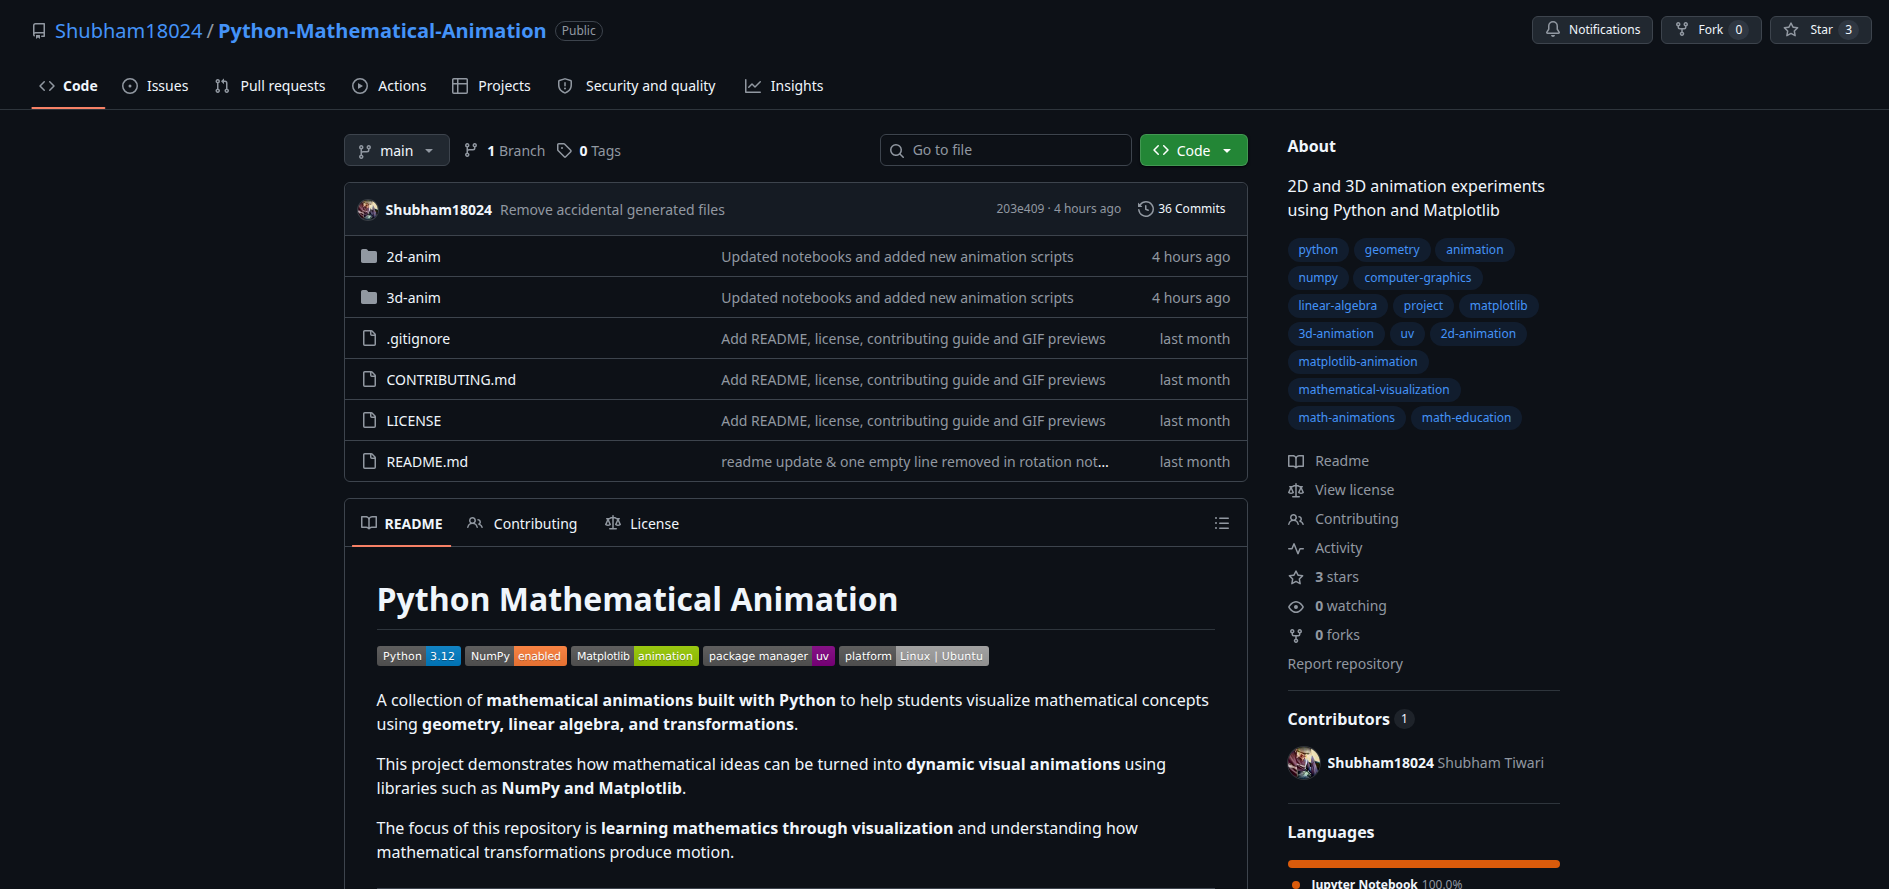
\includegraphics[width=\linewidth, height=0.6\textheight, keepaspectratio]{GITHUB.png}
\end{columns}
\end{frame}

%------------------------------------------------
\begin{frame}{Robust Environment Control: uv}
\begin{itemize}
    \item \textbf{Zero Dependency Issues:} Entire project stack managed via the Rust-based \texttt{uv} manager.
    \item \textbf{Reproducibility:} Isolated environments ensure the code runs flawlessly across Linux, Windows, and Mac.
    \item \textbf{Speed:} Dependency resolution and installation 10-100x faster than standard \texttt{pip}.
\end{itemize}
\vspace{0.3cm}
\centering
\texttt{uv sync} $\rightarrow$ \texttt{uv run jupyter notebook}
\end{frame}
%------------------------------------------------
\begin{frame}{Overcoming Technical Difficulties}
\begin{itemize}
    \item \textbf{CPU-Bound Rendering Limits:} Matplotlib renders on the CPU, causing FPS drops on dense topologies (like the Helicoid). \textit{Solution:} Carefully optimized \texttt{np.linspace} resolution.
    \item \textbf{Z-Buffering (Depth Sorting) Artifacts:} Matplotlib uses a 2D "painter's algorithm" to fake 3D, leading to background polygons bleeding through. \textit{Solution:} Manually enforced viewing angles.
    \item \textbf{Memory Leaks:} Continuous redrawing crashed the RAM. \textit{Solution:} Implemented strict \texttt{ax.clear()} garbage collection per frame.
    \item \textbf{Aspect Ratio Distortion:} Auto-scaling warped 3D rotating spheres into ellipsoids. \textit{Solution:} Hardcoded \texttt{ax.set\_box\_aspect([1,1,1])} to force isometric dimensions.
\end{itemize}
\end{frame}
%------------------------------------------------
\begin{frame}{Future Scope}
\begin{itemize}
    \item \textbf{GPU Migration:} Shifting from CPU-bound Matplotlib to Manim or Three.js for 60 FPS real-time rendering.
    \item \textbf{GUI Development:} Creating a PyQt-based application for students to input their own parametric equations via sliders.
    \item \textbf{Physics Engines:} Integrating SciPy ODE solvers for mass, gravity, and collision detection.
\end{itemize}
\end{frame}

%------------------------------------------------
%------------------------------------------------
\begin{frame}{Conclusion}
\begin{itemize}
\item Mathematics can generate motion
\item Linear algebra defines space
\item Parametrization creates geometry
\item Visualization enhances understanding
\end{itemize}

\vspace{0.5cm}
\centering
\Large{\textbf{Mathematics is not static — it is alive.}}
\end{frame}

%------------------------------------------------
\begin{frame}[allowframebreaks]{References}

\footnotesize

\begin{thebibliography}{9}

\bibitem{friedberg}
Friedberg, S. H., Insel, A. J., \& Spence, L. E. (2019). 
\textit{Linear Algebra} (5th ed.). Pearson Education.

\bibitem{kobayashi}
Kobayashi, S. (2019). 
\textit{Differential Geometry of Curves and Surfaces}. Springer.

\bibitem{loney}
Loney, S. L. (1895). 
\textit{The Elements of Coordinate Geometry}. Macmillan.

\bibitem{kreyszig}
Kreyszig, E. (1989). 
\textit{Introductory Functional Analysis with Applications}. Wiley.

\bibitem{python}
Python Software Foundation (2024). 
\textit{Python Language Reference}.\\
https://docs.python.org/

\bibitem{matplotlib}
Matplotlib Developers (2024). 
\textit{Matplotlib Documentation}.\\
https://matplotlib.org/

\bibitem{numpy}
NumPy Developers (2024). 
\textit{NumPy Documentation}.\\
https://numpy.org/

\end{thebibliography}

\end{frame}

%------------------------------------------------
\begin{frame}{Final Thought}

\begin{center}
\large
\textit{"Nature’s patterns are the most beautiful, but they are all governed by the same mathematical laws. In computer animation, we don't just draw; we simulate the laws of the universe."}
\\[0.3cm]
--- ED Catmull (Founder of Pixar Studios)
\end{center}

\vspace{0.5cm}
\begin{center}
\textbf{Thank You!}
\end{center}

\end{frame}

%------------------------------------------------
\end{document}